\documentclass[11pt]{article}

\usepackage[margin=1in]{geometry}
\usepackage{booktabs}
\usepackage{amsmath}
\usepackage{graphicx}
\usepackage{xcolor}
\usepackage{microtype}
\usepackage{caption}
\usepackage{array}
\usepackage{algorithm}
\usepackage{algpseudocode}
\usepackage[numbers,sort&compress]{natbib}
\usepackage[hidelinks]{hyperref}

\newcommand{\cfg}[1]{\texttt{#1}}
\newcommand{\best}[1]{\textbf{#1}}
\captionsetup{font=small}

\title{\textbf{Benchmark Averages Hide the Failures That Matter:\\
Quantizing ESM-2 for Protein Variant-Effect Prediction}}

% This author list must match the metadata typed into the arXiv submission form
% exactly, or the submission stalls in moderation.
\author{Qing Shao\\[2pt]
Department of Chemical and Materials Engineering\\
University of Kentucky, Lexington, KY 40506}
\date{\today}

\begin{document}
\maketitle

\begin{abstract}
\noindent
We benchmark six numerical precision configurations for ESM-2 protein language
models across three axes --- throughput, memory footprint, and predictive
accuracy --- on two workloads with sharply different characteristics: bulk
embedding extraction and deep mutational scanning (DMS) variant-effect scoring.
For ESM2-3B on an H200, FP8 dynamic quantization (\cfg{fp8\_dyn}) delivers
$1.15\times$ the throughput of bf16 while halving peak memory
($12.63 \to 7.24$\,GB), making it the best configuration for embedding
extraction. The same configuration is a poor choice for DMS scoring, where bf16
in eager mode is fastest at every problem size and quantization is pure
overhead. Accuracy is evaluated on the complete ProteinGym substitution
benchmark --- 201 assays, 2.41M variants, both model scales --- with a paired
bootstrap clustered on protein. Two findings follow. First, fidelity measured
\emph{against fp32}, the metric such studies normally report, predicts the
\emph{magnitude} of the change in real-world accuracy ($r = 0.81$ over 1005
assay/configuration pairs) but not its \emph{sign}: INT4 weight-only
quantization is significantly \emph{beneficial} at 3B and significantly
\emph{harmful} at 650M. Second, and of more practical consequence, no
configuration shifts mean benchmark correlation by more than $0.007$, yet
INT8 dynamic quantization --- indistinguishable from fp32 on that mean
($p = 0.34$) --- takes a single assay from $\rho = 0.591$ to $0.223$. Benchmark
averages conceal precisely the failure that determines whether a configuration
is deployable. We conclude that drift-from-fp32 metrics are sound risk bounds
but unsound quality rankings, that configuration selection should be made on
worst-case rather than mean behaviour, and we report four measurement artifacts
encountered during this study, three of which inverted the result they were
meant to measure.
\end{abstract}

\noindent
\textbf{Keywords:} protein language models; ESM-2; post-training quantization;
variant-effect prediction; ProteinGym; benchmark methodology; FP8; INT8

\section{Introduction}

Quantization is usually presented as a straightforward trade: reduce numerical
precision, gain speed and memory, lose a little accuracy. This framing is
inherited from large autoregressive language models, where it is broadly
correct. We set out to test whether it transfers to ESM-2, a family of protein
language models, and found that essentially every part of it requires
qualification.

ESM-2 is a BERT-style bidirectional \emph{encoder}. It performs a single forward
pass with no KV cache and no autoregressive decode. This places it in a
\textbf{compute-bound} regime rather than the memory-bandwidth-bound regime that
governs LLM inference at batch size 1. The distinction is not academic: the
dominant open-source quantization toolchains (GPTQ, AWQ, bitsandbytes NF4, GGUF)
are all \emph{weight-only}. They store INT4/INT8 weights and dequantize to bf16
immediately before an ordinary bf16 matrix multiply. When the bottleneck is
memory bandwidth, this is a large win. When the bottleneck is arithmetic, as it
is here, it adds work to an already-saturated kernel.

This paper addresses three questions:

\begin{enumerate}
  \item What do the available quantization configurations actually cost and
        deliver on the three axes of speed, memory, and accuracy?
  \item Does the answer depend on the workload? (It does, and the two workloads
        we study prefer opposite configurations.)
  \item Do the fidelity metrics conventionally used to validate quantization
        predict real-world predictive accuracy? (Only partially, and in a way
        that matters.)
\end{enumerate}

\subsection*{Contributions}

\begin{itemize}\setlength{\itemsep}{2pt}
  \item An evaluation of six precision configurations for ESM-2 on the
        \textbf{complete ProteinGym substitution benchmark} --- 201 assays,
        2.41M variants, 40{,}775 masked positions, at two model scales --- rather
        than on drift from the full-precision model or on a handful of assays.
  \item The finding that \textbf{benchmark-mean accuracy is nearly uninformative
        for deployment}. No configuration shifts mean correlation by more than
        $0.007$, while one configuration that passes the mean test at $p=0.34$
        takes a single assay from $\rho = 0.591$ to $0.223$. We argue that
        worst-case single-assay drift, not the mean, is the selection criterion.
  \item A quantitative characterisation of what drift-from-fp32 metrics do and
        do not buy: over 1005 assay/configuration pairs they predict the
        magnitude of ground-truth change ($r = 0.81$) but not its direction,
        which does not even hold its sign between model scales.
  \item The observation that the \textbf{two common ESM-2 workloads prefer
        opposite configurations}, so that a pipeline running both cannot be
        tuned with a single choice.
  \item A documented account of \textbf{four measurement artifacts}, three of
        which inverted the quantity being measured while producing plausible,
        monotonic result tables --- offered as reusable hazards rather than as
        local mistakes.
  \item Open code, per-variant predictions for all 12 model/configuration
        combinations, and per-assay statistics (Section~\ref{sec:avail}).
\end{itemize}

\section{Background and Related Work}

\paragraph{Protein language models.} ESM-2~\cite{lin2023esm2} is a family of
transformer encoders trained with masked language modelling on UniRef, following
ESM-1b~\cite{rives2021}. Architecturally these are BERT-style bidirectional
encoders~\cite{devlin2019bert}: a single forward pass, no KV cache, no
autoregressive decode. \citet{meier2021} established that such models predict
variant effects zero-shot via \emph{masked marginals} --- masking a mutated
position and comparing the log-probabilities of mutant and wild-type residues ---
which is the scoring protocol used throughout this work.

\paragraph{Variant-effect benchmarks.} ProteinGym~\cite{notin2023proteingym}
aggregates deep mutational scanning assays into a standard benchmark; the v1
substitution set used here contains 217 assays spanning 2.47M variants and five
functional categories, including the mega-scale stability measurements of
\citet{tsuboyama2023}. Reporting mean Spearman correlation across assays is the
established summary statistic, and one of our contributions is to show what that
statistic conceals.

\paragraph{Post-training quantization.} The dominant open-source toolchains are
weight-only: GPTQ~\cite{frantar2023gptq} and AWQ~\cite{lin2024awq} store INT4
weights and dequantize before a bf16 matmul, while
LLM.int8()~\cite{dettmers2022llmint8} introduced mixed-precision decomposition to
handle activation outliers. These were designed for autoregressive decoding,
where batch-1 inference is memory-bandwidth-bound and dequantization is
effectively free. Weight--activation (W8A8) schemes and the FP8 E4M3/E5M2
formats~\cite{micikevicius2022fp8} instead reduce arithmetic cost, which is what
a compute-bound encoder requires. We use \texttt{torchao}~\cite{torchao} for all
configurations and PyTorch~2's compiler stack~\cite{ansel2024pytorch2}, whose
Inductor backend emits Triton~\cite{tillet2019triton} kernels; Section~4.1 shows
that the compile mode, not the quantization scheme, determines whether W8A8 is
viable at all. Quantization is also load-bearing for parameter-efficient
fine-tuning~\cite{dettmers2023qlora}, a setting we do not evaluate.

\paragraph{Positioning.} Quantization studies for protein language models are
comparatively rare, and where accuracy is reported it is typically drift against
the full-precision model on a small probe set. Our contribution is to replace
that proxy with the full downstream benchmark at two model scales, and to show
that the proxy is a valid risk bound but an invalid quality ranking.

\section{Experimental Design}

\subsection{Configurations}

Six configurations were evaluated, all applied via \texttt{torchao} to the
encoder \texttt{Linear} layers only:

\begin{table}[htb]
\centering
\caption{Quantization configurations. Weight-only variants target memory; the
dynamic (W8A8) variants also quantize activations and can therefore use
low-precision tensor cores for the matrix multiply itself.}
\small
\begin{tabular}{llp{7.4cm}}
\toprule
Configuration & Class & Description \\
\midrule
\cfg{fp32}     & baseline    & Reference for all fidelity measurements. \\
\cfg{bf16}     & baseline    & The practical production default. \\
\cfg{int8\_wo} & weight-only & INT8 weights, bf16 compute. Memory-oriented. \\
\cfg{int4\_wo} & weight-only & INT4 weights, bf16 compute. Smallest footprint. \\
\cfg{int8\_dyn}& W8A8        & INT8 weights \emph{and} dynamically quantized
                               activations; uses INT8 tensor cores. \\
\cfg{fp8\_dyn} & W8A8        & FP8 (E4M3) weights and activations. Requires
                               compute capability $\geq 8.9$; H200 only. \\
\bottomrule
\end{tabular}
\end{table}

\subsection{Workloads}

\textbf{Bulk embedding extraction.} Large length-bucketed batches under a token
budget, measured in residues per second. This is the compute-bound regime.

\textbf{DMS variant-effect scoring.} The standard ESM masked-marginals protocol:
for each mutated position, mask it and record
$\log p(\text{mut}) - \log p(\text{wt})$ from the resulting distribution. Cost
scales with the \emph{number of mutated positions}, not with the number of
variants, and the masked batch is narrow. This is the latency-bound regime.

Algorithm~\ref{alg:mm} states the scoring procedure as implemented. Two
optimizations, both absent from typical reference implementations, are marked:
only positions carrying a variant are masked (line~\ref{ln:pos}), and the masked
copies are batched rather than run one at a time (line~\ref{ln:batch}). Together
they are worth one to two orders of magnitude on a real assay --- the median
ProteinGym assay mutates 96 positions out of $L=222$ --- and they are applied
identically to every configuration, so they change the absolute cost of the
benchmark without affecting any comparison within it.

\begin{algorithm}[htb]
\caption{Masked-marginals variant scoring, as benchmarked. Cost is
$\lceil |P| / B \rceil$ forward passes and is independent of $|V|$, so an assay
with 16{,}000 variants over 900 positions costs the same as one with 900.}
\label{alg:mm}
\begin{algorithmic}[1]
\Require wild-type sequence $s$, variants $V$, model $f_\theta$, batch size $B$
\Ensure score $\sigma(v)$ for every $v \in V$
\State $M \gets \{\,\text{parse}(v) : v \in V\,\}$
       \Comment{each $v$ is a set of $(\text{wt}, \text{pos}, \text{mut})$ triples}
\For{each $(a, i, b) \in \bigcup M$}
  \State \textbf{assert} $s_i = a$
         \Comment{indexing check; a mismatch is silent and unrecoverable later}
\EndFor
\State $P \gets \{\, i : (a,i,b) \in \bigcup M \,\}$ \label{ln:pos}
       \Comment{\textbf{only} variant-carrying positions, not all $L$}
\For{each chunk $C \subseteq P$ with $|C| = B$} \label{ln:batch}
  \State $X \gets$ $|C|$ copies of tokenize($s$); set $X_{r,\,c_r} \gets \texttt{[MASK]}$
         \Comment{one masked position per row}
  \State $Z \gets f_\theta(X)$ \Comment{single batched forward pass}
  \For{each $r$, with $c_r \in C$}
    \State $\ell_{c_r} \gets \log\mathrm{softmax}\!\left(Z_{r,\,c_r} \text{ in fp32}\right)$
           \Comment{fp32 softmax regardless of compute precision}
  \EndFor
\EndFor
\For{each $v \in V$}
  \State $\sigma(v) \gets \sum_{(a,i,b) \in M_v} \big(\ell_i[b] - \ell_i[a]\big)$
         \Comment{difference of near-equal terms: noise does not cancel}
\EndFor
\end{algorithmic}
\end{algorithm}

The final line is why DMS $\rho$ is the most sensitive fidelity metric we record.
The score is a difference of two nearly equal log-probabilities, so quantization
error in $\ell_i$ does not cancel between the two terms; it is amplified relative
to the signal.

\subsection{Metrics}

Three fidelity metrics were recorded, deliberately ordered by sensitivity:

\begin{enumerate}
  \item \textbf{Embedding cosine similarity} (mean-pooled, excluding special
        tokens and padding). Forgiving: error averages out along the sequence.
  \item \textbf{Logit KL divergence}, per residue. Moderately sensitive.
  \item \textbf{DMS Spearman $\rho$ against fp32.} Most sensitive, because the
        score is a \emph{difference of two near-equal log-probabilities}, so
        quantization noise does not cancel and is amplified relative to signal.
\end{enumerate}

All three are drift-from-fp32 measures. They quantify how far a configuration
moves the answer, not whether it moves toward or away from the truth. To measure
the latter, we added a fourth metric requiring real experimental data:
\textbf{Spearman $\rho$ against wet-lab DMS measurements}, from ProteinGym.

\subsection{Real assay data}

Three ProteinGym substitution assays were selected to span the sequence-length
range, since peak memory during masked-marginals scoring grows with $L$:

\begin{table}[htb]
\centering
\caption{ProteinGym assays used. All 19{,}557 single-substitution variants had
their stated wild-type residue verified against the reference \texttt{target\_seq}
before use; all matched. This check is load-bearing --- an off-by-one in
position indexing does not raise an error, it silently scores the wrong
positions and yields a plausible-looking correlation.}
\small
\begin{tabular}{lrrrl}
\toprule
Assay & $L$ & Singles & Masked positions & Coverage \\
\midrule
\texttt{IF1\_ECOLI\_Kelsic\_2016}     &  72 &  1{,}367 &  72 & 100\% \\
\texttt{BLAT\_ECOLX\_Stiffler\_2015}  & 286 &  4{,}996 & 263 &  92\% \\
\texttt{HSP82\_YEAST\_Flynn\_2019}    & 709 & 13{,}194 & 707 & 100\% \\
\bottomrule
\end{tabular}
\end{table}

\subsection{Full benchmark data}

The three-assay analysis is superseded by a run over the complete ProteinGym
substitution benchmark. All 217 assays were extracted from the
\texttt{ProteinGym\_v1} parquet release and every one passed wild-type
validation across 2{,}465{,}767 variants. The 201 assays fitting ESM-2's
1022-residue context were scored: 2{,}413{,}913 variants over 40{,}775 masked
positions, spanning $L = 37$ to $934$ and five function categories.

The masked-position count, not the variant count, sets the cost: masked-marginals
scoring performs one forward pass per mutated position, so 2.41M variants are
nearly free on top of 40{,}775 forwards.

An earlier three-assay path combined per-assay CSVs from the \texttt{v0.1}
release with wild-type sequences from the \texttt{v1.0} reference file. The two
agree on the 85 assays present in both and diverge elsewhere, including renames.
That is acceptable for three hand-picked assays and unsafe at benchmark scale;
the \texttt{v1} parquet carries \texttt{target\_seq} inline, so scores and
wild-type sequences come from a single release.

\subsection{Statistical treatment}

Ground-truth correlations are compared using a \textbf{paired bootstrap} (2000
resamples). Both the candidate configuration and the fp32 reference are scored
on the \emph{same} resample at each iteration, so shared noise cancels and the
residual is attributable to the configuration. The pairing is not a refinement:
for \cfg{int4\_wo} the paired interval is $8.4\times$ narrower than the unpaired
one, because per-assay $\rho$ spans $0.0$--$0.9$ while the configuration effect is
of order $0.006$. Unpaired, every configuration reads as noise.

The \emph{resampling unit} differs by scale of claim. For a single assay the
unit is the variant, which establishes that a shift is not an artifact of the
variant set. For the full benchmark the unit is the assay, since the claim
becomes one about assays in general. Because the 201 assays cover only 173
distinct proteins, benchmark-level intervals use a \textbf{cluster bootstrap
over proteins}: whole proteins are drawn and all their assays retained, so
correlated replicates cannot count as independent evidence. Clustered and
unclustered intervals agreed to the fourth decimal, which is reported as a
measured result rather than assumed.

Intervals are percentile bootstrap~\cite{efron1993}. They were checked against a
normal approximation ($\bar{d} \pm 1.96\,\mathrm{SE}$) and agree to four decimals
on every configuration, confirming the underlying distribution is near-symmetric
and the percentile method is not distorting the interval. The procedure was
validated on synthetic data with a known answer: a negligible perturbation was
correctly classified as noise, a genuine improvement as real.

Algorithm~\ref{alg:boot} states the benchmark-level test. The pairing is
line~\ref{ln:pair}: one resample index is applied to the candidate and to the
reference \emph{together}. Without it the interval widens by $8.4\times$ for
\cfg{int4\_wo}, because between-assay variance in $\rho$ (spanning $0.0$ to
$0.9$) is two orders of magnitude larger than the configuration effect
($\approx 0.006$), and every configuration is then reported as noise.

\begin{algorithm}[htb]
\caption{Paired cluster bootstrap for $\Delta$(mean $\rho$) against the fp32
reference. Setting $\mathcal{G}$ to singletons recovers the ordinary
assay-level bootstrap; we report both.}
\label{alg:boot}
\begin{algorithmic}[1]
\Require per-assay correlations $\rho^{c}_{a}, \rho^{\text{ref}}_{a}$ for assays
         $a = 1{:}n$; protein clusters $\mathcal{G}$ partitioning the assays;
         $R = 2000$
\Ensure point estimate $\Delta$, 95\% interval, two-sided $p$
\State $\Delta \gets \frac{1}{n}\sum_a \rho^{c}_{a} - \frac{1}{n}\sum_a \rho^{\text{ref}}_{a}$
\For{$r = 1$ \textbf{to} $R$}
  \State draw $|\mathcal{G}|$ clusters from $\mathcal{G}$ with replacement
  \State $S_r \gets$ concatenation of all assays in the drawn clusters
         \Comment{$|S_r|$ varies between replicates}
  \State $d_r \gets \frac{1}{|S_r|}\sum_{a \in S_r}\!\big(\rho^{c}_{a} - \rho^{\text{ref}}_{a}\big)$
         \label{ln:pair}
         \Comment{\textbf{same} $S_r$ indexes both arms}
\EndFor
\State $[\,\ell, u\,] \gets$ 2.5th and 97.5th percentiles of $\{d_r\}$
\State $p \gets 2\min\!\big(\tfrac{1}{R}|\{d_r \le 0\}|,\; \tfrac{1}{R}|\{d_r \ge 0\}|\big)$
       \Comment{floor $2/R = 0.001$; report smaller values as $p < 0.002$}
\State \Return $\Delta$, $[\ell, u]$, $p$; call the effect real iff $0 \notin [\ell, u]$
\end{algorithmic}
\end{algorithm}

\subsection{Hardware and software environment}

\begin{table}[htb]
\centering
\caption{Hardware and software environment. The glibc 2.17 ceiling is what forces torch 2.6.0 and rules out the prebuilt bitsandbytes GPU wheels, so NF4 was unavailable and is absent from the configuration list.}
\small
\begin{tabular}{ll}
\toprule
Component & Detail \\
\midrule
GPU (primary)  & NVIDIA H200, 143\,GB, sm\_90 (FP8 tensor cores) \\
GPU (secondary)& NVIDIA A100, 80\,GB, sm\_80 (no FP8) \\
Driver         & 550.54.14 \\
PyTorch        & 2.6.0+cu124 \\
Attention      & SDPA \\
Compile mode   & \texttt{max-autotune-no-cudagraphs} \\
\bottomrule
\end{tabular}
\end{table}

The cluster runs CentOS 7.6 with glibc 2.17 on every node, including the H200
nodes, which forced several choices. PyTorch moved to \texttt{manylinux\_2\_28}
at version 2.7, making \textbf{2.6.0 the newest installable release}.
\texttt{bitsandbytes} GPU wheels require a newer glibc, so only the CPU-only
0.42.0 installs and its NF4 path is unavailable --- 4-bit quantization therefore
goes through \texttt{torchao}. The system GCC (4.8.5) cannot build Triton's
helper module, so \texttt{torch.compile} fails until \texttt{CC}/\texttt{CXX}
are pointed at GCC 12.1.0. Finally, \texttt{\$HOME} and \texttt{/project} are at
quota, and the Triton, Inductor, HuggingFace, and pip caches all default there;
all were relocated to \texttt{/scratch}. \texttt{torchao} nonetheless works
because its INT8/FP8 paths dispatch to \texttt{torch.\_int\_mm} and
\texttt{torch.\_scaled\_mm}, which live inside PyTorch and support sm\_90.

\section{Results}

\subsection{Compile mode determines whether W8A8 is viable at all}

The single most consequential configuration choice is not the quantization
scheme but the \texttt{torch.compile} mode. Measured on a single ESM2-3B-shaped
feed-forward block, $2560 \to 10240 \to 2560$, at batch $32 \times 512$ on an
A100:

\begin{table}[htb]
\centering
\caption{Only \texttt{max-autotune} allows Inductor to autotune the INT8 Triton
matmuls, which is where the entire W8A8 benefit resides.}
\small
\begin{tabular}{lr}
\toprule
Variant & Time (ms) \\
\midrule
bf16 eager                                   & 7.91 \\
bf16 compiled                                & 7.91 \\
\cfg{int8\_dyn} eager                        & 33.35 \\
\cfg{int8\_dyn} compiled, \texttt{dynamic=True} & 11.73 \\
\cfg{int8\_dyn} compiled, default mode       & 11.48 \\
\cfg{int8\_dyn} \texttt{mode="max-autotune"} & \best{5.43} \\
\bottomrule
\end{tabular}
\end{table}

Measured in eager mode, W8A8 appears $4.2\times$ \emph{slower} than bf16 and
would be discarded. Measured under \texttt{max-autotune} it is $1.46\times$
faster. \texttt{dynamic=True} was avoided because it emits shape-generic kernels
that surrender most of the gain; static shapes are kept manageable by padding to
a fixed multiple of 128. \texttt{torch.\_dynamo.explain} confirms \textbf{zero
graph breaks} for both bf16 and \cfg{int8\_dyn}, establishing this as a
kernel-selection effect rather than a Dynamo fallback.

\subsection{Bulk embedding extraction}

\begin{table}[htb]
\centering
\caption{ESM2-3B, H200, compiled with \texttt{max-autotune-no-cudagraphs}, SDPA
attention, 64 sequences of length 512--1024 under a 16{,}384-token budget.
Reproduced across four independent jobs: bf16 mean 56{,}642 residues/s, range
55{,}941--57{,}422 ($\pm 1.3\%$); fp32 mean 6{,}742, range 6{,}687--6{,}814.}
\small
\begin{tabular}{lrrrrrrr}
\toprule
Config & Weights & Peak & Residues/s & vs bf16 & Emb.\ cos & Logit KL & DMS $\rho_{\text{fp32}}$ \\
       & (GB)    & (GB) &            &         &           &          & \\
\midrule
\cfg{fp32} (ref)  & 10.72 & 25.37 &  6{,}750 & 0.12$\times$ & ---      & ---      & --- \\
\cfg{bf16}        &  5.29 & 12.63 & 57{,}057 & 1.00$\times$ & 0.999949 & 1.17e--04 & 0.9998 \\
\cfg{int8\_wo}    &  2.66 &  8.48 & 54{,}816 & 0.96$\times$ & 0.999959 & 1.05e--04 & 0.9998 \\
\cfg{int8\_dyn}   &  2.65 & \best{7.07} & 59{,}996 & 1.05$\times$ & 0.989592 & 1.40e--02 & 0.9928 \\
\cfg{fp8\_dyn}    &  2.65 &  7.24 & \best{65{,}376} & \best{1.15$\times$} & 0.999920 & 4.60e--04 & 0.9988 \\
\cfg{int4\_wo}    & \best{1.61} &  7.69 &  3{,}813 & 0.07$\times$ & 0.998904 & 1.89e--03 & 0.9975 \\
\bottomrule
\end{tabular}
\end{table}

Three observations. First, the \textbf{fp32 $\to$ bf16 step is worth
$8.4\times$} --- larger than everything quantization adds on top of it, and the
single biggest lever available. Second, \cfg{fp8\_dyn} dominates
\cfg{int8\_dyn}: it is faster ($1.15\times$ vs $1.05\times$) \emph{and}
dramatically more accurate (embedding cosine 0.999920 vs 0.989592; logit KL
$4.6\times10^{-4}$ vs $1.4\times10^{-2}$), surrendering only 0.17\,GB of peak
memory. FP8's E4M3 format has far greater dynamic range than INT8 at the same
bit width, which matters because transformer activations contain outliers.
Third, \cfg{int4\_wo} is a trap for inference: $0.07\times$ throughput and
\emph{worse} peak memory (7.69\,GB) than \cfg{fp8\_dyn} (7.24\,GB) despite 40\%
smaller weights, because the dequantization path allocates transient buffers.
Its value lies elsewhere, as a QLoRA base.

Separately, length-bucketed batching reduced padding waste from 25.0\% (naive
fixed-size batching) to \textbf{0.0\%}. This is free and costs no accuracy ---
a larger effect than several of the quantization differences in the table.

\subsection{DMS scoring: the opposite conclusion}

\begin{table}[htb]
\centering
\caption{DMS scoring throughput, ESM2-3B, uncompiled. bf16 wins at every problem
size; quantization is pure overhead in this regime.}
\small
\begin{tabular}{lrrr}
\toprule
Config & \multicolumn{3}{c}{Variants/s} \\
\cmidrule(lr){2-4}
       & IF1 ($L{=}72$) & BLAT ($L{=}286$) & HSP82 ($L{=}709$) \\
\midrule
\cfg{bf16}      & \best{6{,}979} & \best{3{,}573} & \best{1{,}357} \\
\cfg{int8\_wo}  & 4{,}830 & 2{,}511 & 1{,}066 \\
\cfg{fp8\_dyn}  & 1{,}813 & 1{,}796 & 1{,}103 \\
\cfg{fp32}      & 1{,}460 &   447 &   187 \\
\cfg{int8\_dyn} &   410 &   382 &   299 \\
\cfg{int4\_wo}  & 1{,}045 &   282 &   112 \\
\bottomrule
\end{tabular}
\end{table}

bf16 is fastest at every assay size, and \cfg{int8\_dyn} --- the second-fastest
configuration for bulk extraction --- is up to $17\times$ slower here. The
masked batch (n\_positions $\times$ $L$) is too small to contain a matrix
multiply large enough for low precision to pay for its quantize/dequantize
overhead.

Notably, \cfg{fp8\_dyn} closes on bf16 as the assay grows: $0.26\times$,
$0.50\times$, $0.81\times$ of bf16 throughput at $L = 72, 286, 709$
respectively. Its overhead is fixed per call while real work scales, so at
$L=709$ it costs 20\% throughput for 43\% less memory --- a defensible trade
that is indefensible at $L=72$.

\subsection{Memory during DMS scoring}

\begin{table}[htb]
\centering
\caption{Peak device memory during DMS scoring. Weights account for
approximately 90\% of peak even at $L=709$ (bf16: 5.29\,GB weights against
0.59\,GB activations).}
\small
\begin{tabular}{lrrrr}
\toprule
Config & Weights (GB) & Peak $L{=}72$ & Peak $L{=}286$ & Peak $L{=}709$ \\
\midrule
\cfg{fp32}      & 10.72 & 10.87 & 11.19 & 11.85 \\
\cfg{bf16}      &  5.29 &  5.38 &  5.55 &  5.88 \\
\cfg{int8\_wo}  &  2.66 &  2.77 &  2.92 &  3.25 \\
\cfg{int8\_dyn} &  2.65 &  2.87 &  2.91 &  3.36 \\
\cfg{fp8\_dyn}  &  2.65 &  2.76 &  2.96 &  3.35 \\
\cfg{int4\_wo}  & \best{1.61} & \best{1.70} & \best{1.87} & \best{2.20} \\
\bottomrule
\end{tabular}
\end{table}

This is the reverse of the bulk-extraction situation. Masked-marginals scoring
keeps the batch narrow, so the $O(L^2)$ attention term never dominates and
weights remain roughly 90\% of peak memory even at $L=709$. Quantization
therefore addresses almost all of DMS peak memory, and \cfg{int4\_wo} gives the
smallest footprint at every length --- $2.7\times$ below bf16.

\subsection{Ground-truth accuracy on ProteinGym}
\label{sec:gt}

\begin{table}[htb]
\centering
\caption{Spearman correlation against experimental measurements, ESM2-3B.
$\Delta$ is the change from fp32, with a 2000-sample paired bootstrap over
variants. ``Real'' indicates the 95\% confidence interval excludes zero.}
\small
\begin{tabular}{llrrrl}
\toprule
Assay & Config & $\rho_{\text{expt}}$ & $\Delta$ vs fp32 & 95\% CI of $\Delta$ & Verdict \\
\midrule
IF1        & \cfg{fp32}      & 0.5561 & (ref)    &                      &  \\
($n{=}1367$)& \cfg{bf16}      & 0.5543 & $-0.0018$ & $[-0.0027, -0.0009]$ & \textbf{real} \\
           & \cfg{int8\_wo}  & 0.5570 & $+0.0009$ & $[-0.0003, +0.0021]$ & noise \\
           & \cfg{int8\_dyn} & 0.5504 & $-0.0057$ & $[-0.0124, +0.0013]$ & noise \\
           & \cfg{fp8\_dyn}  & 0.5584 & $+0.0023$ & $[-0.0022, +0.0067]$ & noise \\
           & \cfg{int4\_wo}  & 0.5394 & $\mathbf{-0.0167}$ & $[-0.0263, -0.0074]$ & \textbf{real} \\
\midrule
BLAT       & \cfg{fp32}      & 0.5893 & (ref)    &                      &  \\
($n{=}4996$)& \cfg{bf16}      & 0.5896 & $+0.0003$ & $[-0.0003, +0.0009]$ & noise \\
           & \cfg{int8\_wo}  & 0.5913 & $+0.0019$ & $[+0.0011, +0.0029]$ & \textbf{real} \\
           & \cfg{int8\_dyn} & 0.6160 & $\mathbf{+0.0266}$ & $[+0.0219, +0.0315]$ & \textbf{real} \\
           & \cfg{fp8\_dyn}  & 0.6088 & $\mathbf{+0.0194}$ & $[+0.0161, +0.0229]$ & \textbf{real} \\
           & \cfg{int4\_wo}  & 0.6388 & $\mathbf{+0.0495}$ & $[+0.0433, +0.0561]$ & \textbf{real} \\
\midrule
HSP82      & \cfg{fp32}      & 0.2931 & (ref)    &                      &  \\
($n{=}13194$)& \cfg{bf16}    & 0.2933 & $+0.0002$ & $[-0.0002, +0.0005]$ & noise \\
           & \cfg{int8\_wo}  & 0.2933 & $+0.0002$ & $[-0.0002, +0.0007]$ & noise \\
           & \cfg{int8\_dyn} & 0.2937 & $+0.0006$ & $[-0.0020, +0.0028]$ & noise \\
           & \cfg{fp8\_dyn}  & 0.2944 & $+0.0012$ & $[-0.0003, +0.0027]$ & noise \\
           & \cfg{int4\_wo}  & 0.2904 & $-0.0027$ & $[-0.0057, +0.0002]$ & noise \\
\bottomrule
\end{tabular}
\end{table}

Two findings emerge, and the second qualifies the first.

\paragraph{Quantization does not systematically degrade variant-effect
accuracy.} Of the 15 assay/configuration pairs, 11 shifts are upward. Most are
statistically indistinguishable from zero. Strikingly, \cfg{int4\_wo} --- the
worst configuration on every fidelity metric --- produces the \emph{best}
agreement with experiment on BLAT ($+0.0495$, CI $[+0.0433, +0.0561]$). This
survives the bootstrap and is not a resampling artifact.

\paragraph{Fidelity-vs-fp32 predicts the magnitude of the shift, not its sign.}
Across all 15 pairs, the correlation between fidelity loss
($1 - \rho_{\text{fp32}}$) and the absolute ground-truth shift is
$r = 0.87$ (Pearson), $\rho = 0.76$ (Spearman). But \cfg{int4\_wo} moves
$+0.0495$ on BLAT and $-0.0167$ on IF1. The direction is a property of the
assay, not of the configuration, and is not predictable from any
drift-from-fp32 measurement.

The practical consequence is that \cfg{bf16} and \cfg{int8\_wo} shift
ground-truth agreement by at most 0.002 on any assay tested --- below anything
an experiment could resolve --- and are therefore safe. \cfg{int4\_wo} is a
$\pm 0.05$ gamble on an unknown sign.

This supersedes an earlier conclusion drawn from a synthetic 40-residue mutational
scan, which ranked \cfg{int8\_dyn} ($\rho_{\text{fp32}} = 0.9928$) as risky and
\cfg{fp8\_dyn} ($0.9988$) as clearly safer. Both numbers were correct; neither
predicted experimental accuracy. On BLAT the ``risky'' configuration gained
$+0.027$.

We note that the assay itself matters far more than any quantization decision:
$\rho_{\text{expt}}$ ranges from 0.29 (HSP82) to 0.59 (BLAT) at 3B. Choosing
which assay to trust is a $2\times$ effect; choosing a quantization
configuration is a $1\%$ effect.

\subsection{Model-scale consistency}

The same three assays were run on ESM2-650M. The qualitative picture holds:
bf16 fastest, \cfg{int8\_dyn} slowest, ground-truth shifts small. The largest
650M shift was $-0.0063$ (\cfg{int8\_dyn} on IF1) against $\rho_{\text{fp32}}$
of 0.9954. The larger and more clearly significant shifts at 3B indicate that
sensitivity to quantization grows with model size, so 650M results should not be
extrapolated to 3B without checking.

An incidental observation deserves note, because it bears directly on how much
any of this matters. The fp32 650M model correlates with experiment
\emph{better} than the fp32 3B model on two of the three assays:

\begin{table}[htb]
\centering
\caption{Ground-truth correlation by model scale on the three-assay subset. The 0.14 BLAT gap prompted the inference that model choice dominates precision choice; Section~\ref{sec:full} shows it does not generalise.}
\small
\begin{tabular}{lrrr}
\toprule
Assay & 650M $\rho_{\text{expt}}$ & 3B $\rho_{\text{expt}}$ & Difference \\
\midrule
IF1   & 0.5987 & 0.5561 & $-0.0426$ \\
BLAT  & 0.7315 & 0.5893 & $-0.1422$ \\
HSP82 & 0.2648 & 0.2931 & $+0.0283$ \\
\bottomrule
\end{tabular}
\end{table}

The BLAT gap of $0.14$ is roughly \emph{three times} the largest effect any
quantization configuration produced in this study. Model selection dominates
precision selection by a wide margin, and the assumption that the larger
checkpoint is the more accurate one does not hold uniformly here.

\emph{This inference does not survive Section~\ref{sec:full}.} Over 201 assays
the two models are statistically indistinguishable ($p=0.35$). The BLAT gap is
real for BLAT and does not generalise --- the same error, made the same way, as
the \cfg{int4\_wo} result three subsections above.

\subsection{The full benchmark: 201 assays}
\label{sec:full}

Every accuracy conclusion above rests on three assays. Three is enough to
establish that an effect exists on a particular assay and not enough to
establish anything about assays in general, because the unit that varies ---
the assay --- is held fixed. The whole ProteinGym substitution benchmark was
therefore run: all 217 assays validated, the 201 within ESM-2's 1022-residue
context scored, 2{,}413{,}913 variants over 40{,}775 masked positions, six
configurations, two model scales. 3.1 GPU-hours at 3B.

Two changes to the statistical treatment follow from the larger sample. The
resampling unit becomes the \textbf{assay} rather than the variant, since the
question is now whether a configuration degrades prediction in general. And
because the 201 assays cover only 173 distinct proteins --- \texttt{BLAT\_ECOLX}
appears four times --- the reported interval is a \textbf{cluster bootstrap over
proteins}, which prevents correlated replicates from counting as independent
evidence. The two intervals turned out to agree to the fourth decimal, so the
clustering was immaterial here; it is reported because that had to be measured
rather than assumed.

\begin{table}[htb]
\centering
\caption{Mean Spearman against experiment over 201 assays. Bold marks intervals
excluding zero under the protein-clustered paired bootstrap. Note that
\cfg{int4\_wo} is significant in \emph{opposite directions} on the two model
scales. This is not driven by a handful of outliers: \cfg{int4\_wo} is worse
than fp32 on 143 of 201 assays at 650M and on only 91 of 201 at 3B.}
\small
\begin{tabular}{lrrlrrl}
\toprule
& \multicolumn{3}{c}{ESM2-3B} & \multicolumn{3}{c}{ESM2-650M} \\
\cmidrule(lr){2-4}\cmidrule(lr){5-7}
Config & $\bar{\rho}$ & $\Delta$ & 95\% CI & $\bar{\rho}$ & $\Delta$ & 95\% CI \\
\midrule
fp32              & 0.4398 & ---     & (ref)              & 0.4459 & ---     & (ref) \\
\cfg{bf16}        & 0.4399 & $+0.0002$ & $[-0.0001,+0.0004]$ & 0.4460 & $+0.0000$ & $[-0.0003,+0.0004]$ \\
\cfg{int8\_wo}    & 0.4399 & $+0.0001$ & $[-0.0002,+0.0005]$ & 0.4457 & $-0.0002$ & $[-0.0006,+0.0002]$ \\
\cfg{fp8\_dyn}    & 0.4403 & $+0.0005$ & $[-0.0007,+0.0017]$ & 0.4452 & $-0.0008$ & $[-0.0020,+0.0005]$ \\
\cfg{int8\_dyn}   & 0.4376 & $-0.0021$ & $[-0.0072,+0.0017]$ & 0.4440 & $\mathbf{-0.0020}$ & $[-0.0032,-0.0009]$ \\
\cfg{int4\_wo}    & 0.4435 & $\mathbf{+0.0037}$ & $[+0.0007,+0.0068]$ & 0.4395 & $\mathbf{-0.0064}$ & $[-0.0105,-0.0018]$ \\
\bottomrule
\end{tabular}
\end{table}

\subsubsection*{The benchmark mean is the wrong safety criterion}

Every $\Delta$ in that table is below $0.007$. The per-assay tail is not
(Figure~\ref{fig:tail}).

\begin{figure}[t]
\centering
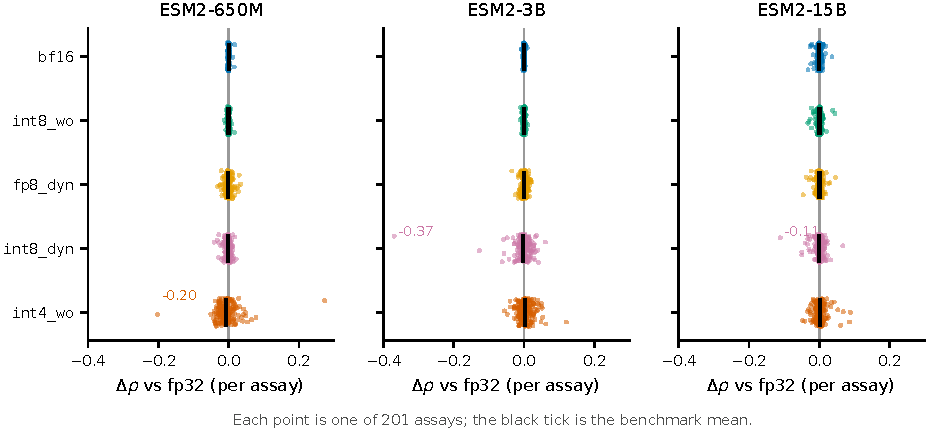
\includegraphics[width=\textwidth]{fig_tail.pdf}
\caption{Per-assay change in ground-truth correlation for each configuration,
across all 201 ProteinGym assays and both model scales. Black ticks mark the
benchmark mean, which is within $0.007$ of zero everywhere. \cfg{bf16} and
\cfg{int8\_wo} are tight at every assay; \cfg{int8\_dyn} and \cfg{int4\_wo} have
means that are equally unremarkable and tails that reach $-0.37$ and $-0.20$.
Selection on the mean cannot distinguish these cases; selection on the tail
separates them immediately.}
\label{fig:tail}
\end{figure}

\begin{table}[htb]
\centering
\caption{Worst single-assay change in ground-truth correlation, and count of
assays moving by more than $0.05$, out of 201.}
\small
\begin{tabular}{lrrrr}
\toprule
& \multicolumn{2}{c}{ESM2-3B} & \multicolumn{2}{c}{ESM2-650M} \\
\cmidrule(lr){2-3}\cmidrule(lr){4-5}
Config & worst $\Delta$ & $|\Delta|>0.05$ & worst $\Delta$ & $|\Delta|>0.05$ \\
\midrule
\cfg{bf16}      & $-0.0072$ & 0 & $-0.0040$ & 0 \\
\cfg{int8\_wo}  & $-0.0106$ & 0 & $-0.0120$ & 0 \\
\cfg{fp8\_dyn}  & $-0.0344$ & 0 & $-0.0316$ & 0 \\
\cfg{int8\_dyn} & $\mathbf{-0.3688}$ & 6 & $-0.0411$ & 0 \\
\cfg{int4\_wo}  & $-0.0556$ & 5 & $\mathbf{-0.2024}$ & 6 \\
\bottomrule
\end{tabular}
\end{table}

\cfg{int8\_dyn} at 3B is indistinguishable from fp32 on the benchmark mean
($\Delta=-0.0021$, $p=0.34$) while destroying
\texttt{UBR5\_HUMAN\_Tsuboyama\_2023\_1I2T}, where correlation with experiment
falls from $0.591$ to $0.223$ at $\rho_{\text{fp32}}=0.393$. A configuration can
pass the benchmark average and be unusable on the one protein a given project
cares about. This is the practical result of the whole study: benchmark-mean
significance testing answers a question about populations, and deployment is a
question about a specific instance.

\subsubsection*{What the larger sample changed}

\textbf{The three-assay verdict was backwards.} Section~\ref{sec:gt} concluded
that quantization does not systematically degrade variant-effect accuracy, on
the evidence that 11 of 15 shifts were upward and that \cfg{int4\_wo} gained
$+0.0495$ on BLAT. At benchmark scale \cfg{int4\_wo} is significant in opposite
directions on the two model scales. Both measurements were correct; the
generalisation from three assays was not.

\textbf{Fidelity predicts magnitude, not direction.} Across
1005 assay/configuration pairs, $r(1-\rho_{\text{fp32}},|\Delta|) = 0.81$ at 3B
and $0.74$ at 650M, confirming the $0.87$ estimated from 15 pairs. The
\emph{signed} correlation is $-0.58$ at 3B and $+0.10$ at 650M --- inconsistent
in sign between model scales, and therefore useless for prediction.
$\rho_{\text{fp32}}$ remains the correct cheap screen, bounding how far an answer
can move while saying nothing about which way (Figure~\ref{fig:fidelity}).

\begin{figure}[t]
\centering
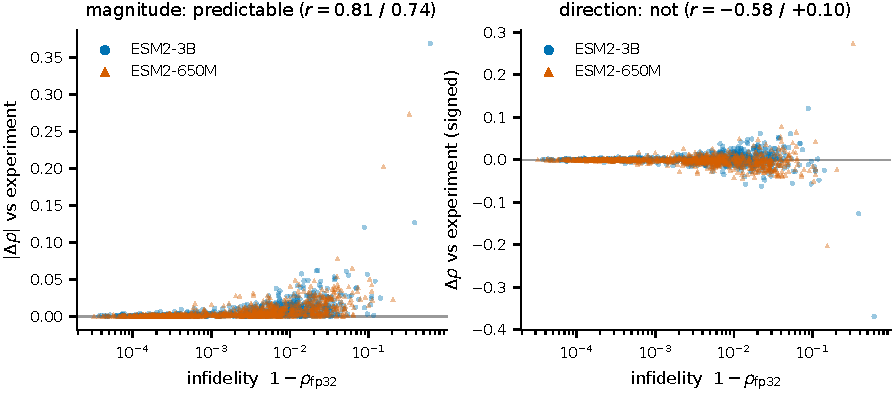
\includegraphics[width=\textwidth]{fig_fidelity.pdf}
\caption{Drift from fp32 against change in ground-truth correlation, over 1005
assay/configuration pairs per model. \emph{Left:} infidelity bounds the
magnitude of the change --- the envelope widens monotonically, and nothing far
from fp32 is reliably close to it on the ground truth. \emph{Right:} the same
data, signed. The distribution is a symmetric funnel rather than a trend, and
the correlation reverses sign between model scales ($-0.58$ at 3B, $+0.10$ at
650M). A small drift is therefore a valid safety certificate, while a large
drift is not evidence of a worse model.}
\label{fig:fidelity}
\end{figure}

\textbf{Damage concentrates where the model is weakest.} \cfg{int4\_wo}'s cost is
monotone in MSA depth at \emph{both} model scales: low $<$ medium $<$ high, with
$-0.0174$ on low-depth assays against $-0.0042$ on high-depth at 650M.
Quantization does most harm where there is least evolutionary signal to lose.
This is the only stratification we find that replicates across scale --- the
breakdown by function category does not, and neither is a distinction three
assays can support. Table~\ref{tab:strata} gives both.

\begin{table}[htb]
\centering
\caption{Mean $\rho$ against experiment, stratified by ProteinGym function
category and by MSA depth. \cfg{bf16}, \cfg{int8\_wo} and \cfg{fp8\_dyn} track
fp32 in every stratum. \cfg{int4\_wo} does not. Its deviations by \emph{function
category} do not transfer across model scale --- Binding is its worst stratum at
650M ($-0.018$) and its second-best at 3B ($+0.005$) --- so category-level
behaviour is no more predictable than the overall sign. Its ordering by
\emph{MSA depth} does transfer, and is monotone at both scales: low $<$ medium
$<$ high ($-0.017 < -0.005 < -0.004$ at 650M, $-0.001 < +0.001 < +0.010$ at 3B).
Quantization costs most where the model has least evolutionary signal to work
with, and that is the one stratification here that replicates.}
\label{tab:strata}
\small
\begin{tabular}{lrrrrrr}
\toprule
Stratum & \cfg{fp32} & \cfg{bf16} & \cfg{int8\_wo} & \cfg{fp8\_dyn} & \cfg{int8\_dyn} & \cfg{int4\_wo} \\
\midrule
\multicolumn{7}{l}{\emph{ESM2-3B}} \\
\quad Activity          & 0.4269 & 0.4271 & 0.4274 & 0.4267 & 0.4270 & 0.4287 \\
\quad Binding           & 0.3392 & 0.3396 & 0.3400 & 0.3440 & 0.3405 & 0.3441 \\
\quad Expression        & 0.4288 & 0.4288 & 0.4293 & 0.4294 & 0.4356 & 0.4270 \\
\quad OrganismalFitness & 0.4006 & 0.4005 & 0.4006 & 0.4005 & 0.3990 & 0.4003 \\
\quad Stability         & 0.5091 & 0.5095 & 0.5089 & 0.5097 & 0.5023 & 0.5192 \\
\quad MSA depth: low    & 0.3264 & 0.3265 & 0.3272 & 0.3261 & 0.3239 & 0.3253 \\
\quad MSA depth: high   & 0.4874 & 0.4876 & 0.4879 & 0.4894 & 0.4888 & 0.4971 \\
\addlinespace
\multicolumn{7}{l}{\emph{ESM2-650M}} \\
\quad Activity          & 0.4332 & 0.4329 & 0.4327 & 0.4315 & 0.4312 & 0.4217 \\
\quad Binding           & 0.3560 & 0.3571 & 0.3565 & 0.3562 & 0.3542 & 0.3376 \\
\quad Expression        & 0.4398 & 0.4397 & 0.4398 & 0.4382 & 0.4390 & 0.4398 \\
\quad OrganismalFitness & 0.3960 & 0.3959 & 0.3959 & 0.3945 & 0.3951 & 0.3844 \\
\quad Stability         & 0.5233 & 0.5235 & 0.5230 & 0.5239 & 0.5200 & 0.5258 \\
\quad MSA depth: low    & 0.3180 & 0.3184 & 0.3186 & 0.3181 & 0.3177 & 0.3006 \\
\quad MSA depth: high   & 0.5176 & 0.5175 & 0.5171 & 0.5175 & 0.5151 & 0.5134 \\
\bottomrule
\end{tabular}
\end{table}

\subsubsection*{Speed and memory over the whole benchmark}

\begin{table}[htb]
\centering
\caption{Full 201-assay benchmark, ESM2-3B on one H200, uncompiled. Wall-clock
is summed scoring time over all assays.}
\small
\begin{tabular}{lrrrr}
\toprule
Config & Wall-clock & Positions/s & Peak RAM (median) & Peak RAM (max) \\
\midrule
fp32            & 45.0 min & 25.6  & 11.10 GB & 12.20 GB \\
\cfg{bf16}      & \textbf{7.3 min} & \textbf{200.6} & 5.50 GB & 6.05 GB \\
\cfg{int8\_wo}  & 9.2 min  & 139.3 & 2.87 GB & 3.42 GB \\
\cfg{fp8\_dyn}  & 10.2 min & 89.2  & 2.90 GB & 3.56 GB \\
\cfg{int8\_dyn} & 40.0 min & 20.1  & 2.94 GB & 3.51 GB \\
\cfg{int4\_wo}  & 73.8 min & 17.3  & \textbf{1.82 GB} & \textbf{2.37 GB} \\
\bottomrule
\end{tabular}
\end{table}

The DMS recommendation from three assays survives and strengthens: \cfg{bf16}
eager, $6.2\times$ faster than fp32 end-to-end, with ground-truth agreement never
moving more than $0.018$ across 402 assay/model pairs. \cfg{int8\_wo} is the
memory fallback at 69\% of bf16 speed and maximum drift $0.016$. \cfg{int8\_dyn}
and \cfg{int4\_wo} are not trade-offs for this workload --- they are slower than
bf16 \emph{and} carry a catastrophic tail.

\section{Reproducibility Pitfalls in Quantization Benchmarking}
\label{sec:pitfalls}

We document four measurement defects encountered during this study. They are
included in the main text, unusually for a paper, because they bear directly on
its thesis: three of the four produced clean, monotonic, plausible result tables
while measuring the wrong quantity, and each would have supported a confident and
wrong recommendation. A reader who accepts our argument that benchmark averages
can mislead should also want to know how the underlying measurements can
mislead. All four are properties of the standard tooling rather than of this
codebase, and we expect them to recur in any comparable study.

\subsection{Compile cost inside the timed region (three occurrences)}

The DMS throughput column initially ranked \cfg{fp32} fastest and \cfg{fp8\_dyn}
slowest --- an exact inversion of the bulk-throughput column. Two successive
fixes failed. Direct instrumentation finally established the cause. On
650M/A100 with a 40-residue wild type over 11 masked positions:

\begin{table}[htb]
\centering
\caption{Compilation cost inside the timed region. A single forward pass at the DMS input shape costs 15\,s to autotune and 28\,ms to execute, so a timed region containing compilation ranks configurations by their number of Triton kernel candidates rather than by their speed.}
\small
\begin{tabular}{lr}
\toprule
Measurement & Time \\
\midrule
eager, one forward at shape $(11, 42)$        & 27.9\,ms \\
eager, full \texttt{masked\_marginals} pass   & 0.03\,s \\
compiled, one forward at shape $(11, 42)$     & \best{15{,}138.1\,ms} \\
\bottomrule
\end{tabular}
\end{table}

DMS scoring uses a much smaller input shape than the bulk-throughput batches,
and under \texttt{max-autotune} each new shape costs roughly 15\,s to autotune.
At this batch size that cost recurs rather than amortizing. The timed region was
therefore measuring \emph{autotune cost}, and ranking configurations by their
number of Triton kernel candidates --- \cfg{fp32} had the fewest and appeared
fastest, \cfg{fp8\_dyn} had 98 and appeared slowest. The fix was to score DMS
against the uncompiled module.

This has a consequence beyond the benchmark: for short wild-type sequences with
few mutated positions, \texttt{max-autotune} is actively counterproductive in
production, not merely in measurement.

The same class of defect appeared earlier in the bulk-throughput path, where
warming up on only a prefix of the batches left recompilation for unseen length
buckets inside the timed region.

\subsection{Peak memory attributed to the wrong model}

Peak memory during DMS scoring was reported as follows, with the activation
overhead implied by subtracting weights:

\begin{table}[htb]
\centering
\caption{The peak-memory artifact. Each configurations measured peak contains the previous configurations weights, which surfaces as bf16 apparently needing more peak memory than fp32.}
\small
\begin{tabular}{lrrr}
\toprule
Config & Weights (GB) & Peak (GB) & Implied overhead \\
\midrule
\cfg{fp32}      & 2.49 & 2.56 & $+0.07$ \\
\cfg{bf16}      & 1.21 & 3.74 & $+2.53 \approx$ fp32's weights \\
\cfg{int8\_wo}  & 0.61 & 1.86 & $+1.25 \approx$ bf16's weights \\
\cfg{int8\_dyn} & 0.61 & 1.26 & $+0.65 \approx$ int8\_wo's weights \\
\bottomrule
\end{tabular}
\end{table}

Each configuration's peak included the \emph{previous} configuration's weights,
producing the visible absurdity of bf16 requiring more peak memory than fp32.
The cleanup helper deleted only its own local reference to the model; the caller
retained a binding. Because \texttt{nn.Module} graphs contain reference cycles,
dropping the last reference does not free them by reference counting alone ---
they persist as cyclic garbage until a collection runs. Inserting an explicit
\texttt{gc.collect()} before each peak-memory reset corrected it; overhead
became a consistent 0.04--0.07\,GB.

The bulk-throughput memory column was verified unaffected: bf16's measured
overhead there was $+7.34$\,GB, which cannot contain fp32's 10.72\,GB of
weights.

\subsection{Silent argument leakage in the job script}

A batch script used \texttt{shift 3 || true}. When fewer than three positional
arguments are supplied, \texttt{shift 3} fails, \texttt{|| true} suppresses the
failure, and the arguments remain in \texttt{"\$@"} --- where they were appended
to the Python invocation as stray arguments. Relying on a default for the third
argument was sufficient to trigger it.

\subsection{Common thread}

Three of the four defects shared a signature: a cost that belonged outside the
measurement leaked inside it, and the resulting ranking was plausible enough to
be believed. In each case the tell was a result that inverted or contradicted a
neighbouring measurement. We would emphasise that a benchmark producing a
\emph{clean, monotonic, plausible} table is not thereby correct; the memory bug
produced exactly such a table for several runs.

\section{Discussion}

\subsection{The two workloads want opposite configurations}

This is the principal practical finding.

\textbf{Bulk embedding extraction} is compute-bound: large batches, large GEMMs.
Quantization pays. \cfg{fp8\_dyn} with \texttt{max-autotune} wins on all three
axes --- $1.15\times$ bf16 throughput, weights $5.29 \to 2.65$\,GB, peak
$12.63 \to 7.24$\,GB, with accuracy indistinguishable from bf16.

\textbf{DMS variant-effect scoring} is latency-bound: the masked batch is small,
no GEMM is large enough for low precision to help, and per-linear
quantize/dequantize overhead is pure loss. bf16 in eager mode is fastest at
every problem size, and \texttt{max-autotune} is actively harmful.

Applying the embedding-optimized configuration to DMS scoring makes it up to an
order of magnitude slower. Because both workloads commonly appear in the same
pipeline, this is a live risk rather than a theoretical one.
Figure~\ref{fig:pareto} shows the two frontiers side by side.

\begin{figure}[t]
\centering
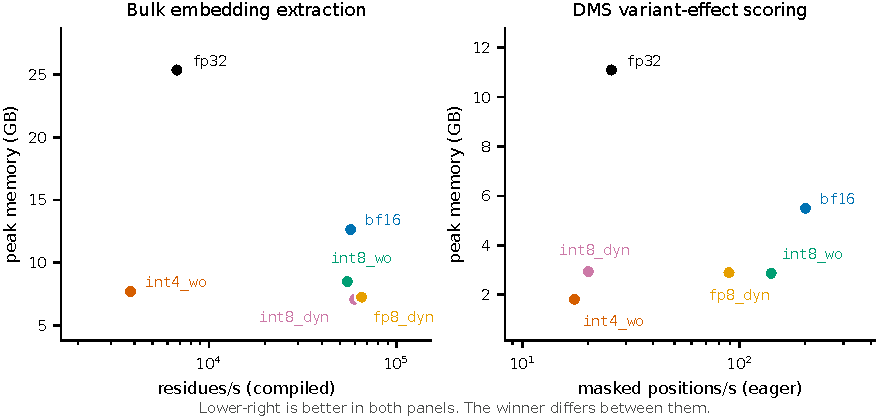
\includegraphics[width=\textwidth]{fig_pareto.pdf}
\caption{Speed--memory frontiers for the two workloads, ESM2-3B on one H200;
lower-right is better in both panels. \emph{Left:} bulk embedding extraction
under \texttt{max-autotune}, where \cfg{fp8\_dyn} is fastest and near-smallest.
\emph{Right:} DMS scoring over the full 201-assay benchmark in eager mode, where
the same configuration is $2.2\times$ slower than \cfg{bf16} and the ranking is
substantially reordered. No single configuration is preferred by both.}
\label{fig:pareto}
\end{figure}

\subsection{On the interpretation of fidelity metrics}
\label{sec:fidelity}

The conventional validation practice --- quantize, measure drift against the
full-precision model, accept if drift is small --- is sound as a
\emph{risk bound}. Our data support the bound at scale: over 1005 assay/
configuration pairs, fidelity loss correlates with the magnitude of ground-truth
change at $r = 0.81$ (3B) and $0.74$ (650M), consistent with the $0.87$ first
estimated from 15 pairs.

It is not sound as a \emph{quality ranking}. A configuration with larger drift
is not thereby less accurate against reality; it is merely less predictable. The
signed correlation is $-0.58$ at 3B and $+0.10$ at 650M --- it does not even
hold its sign between model scales.

A tempting misreading of our BLAT result is that quantization acts as beneficial
regularization. We do not endorse this, and the full benchmark settles it:
\cfg{int4\_wo} is significantly \emph{positive} at 3B and significantly
\emph{negative} at 650M. A configuration cannot be genuinely more accurate than
the reference from which it is derived in any way one could rely on in advance.

\subsection{Averages conceal the failure that matters}

The benchmark-mean result is that no configuration changes mean ground-truth
correlation by more than $0.007$. Read alone, that licenses any configuration on
the list. It should not.

\cfg{int8\_dyn} at 3B is statistically indistinguishable from fp32 on the mean
($p = 0.34$) and takes one assay from $\rho = 0.591$ to $0.223$. A practitioner
does not deploy against the mean of 201 assays; they deploy against one protein.
The benchmark mean answers whether a configuration is safe \emph{on average over
targets}, which is a claim about a population, while the operative question is
whether it is safe on a specific target.

The practical consequence is that the tail statistics --- worst-case single-assay
drift, and the count of assays exceeding a tolerance --- are the numbers to
select on, and they separate the configurations far more sharply than the means
do. On that criterion \cfg{bf16} and \cfg{int8\_wo} are safe (no assay beyond
$0.018$ across 402 assay/model pairs), \cfg{fp8\_dyn} is nearly so ($0.034$), and
\cfg{int8\_dyn} and \cfg{int4\_wo} are not.

\subsection{Recommendations}

\begin{table}[htb]
\centering
\caption{Configuration recommendations by situation. The first two rows differ because the two workloads sit in different bottleneck regimes, not because of any accuracy difference.}
\small
\begin{tabular}{ll}
\toprule
Situation & Recommendation \\
\midrule
Bulk embedding extraction (H200) & \cfg{fp8\_dyn} + \texttt{max-autotune-no-cudagraphs} \\
Bulk embedding extraction (A100) & \cfg{int8\_wo}; \cfg{int8\_dyn} costs real accuracy \\
DMS / variant effect scoring     & \cfg{bf16}, eager, no compile \\
DMS under memory pressure        & \cfg{int8\_wo} (2.87 vs 5.50\,GB; 69\% of bf16 speed) \\
Minimum memory footprint         & \cfg{int4\_wo}, only if a $-0.20$ single-assay \\
                                 & \quad collapse is acceptable; validate on your target \\
QLoRA fine-tuning base           & \cfg{int4\_wo} (1.61\,GB weights) \\
V100 / sm\_70 hardware           & Quantization buys memory only, never speed \\
\bottomrule
\end{tabular}
\end{table}

Two non-quantization measures outweigh most of the above. Moving from fp32 to
bf16 is worth $8.4\times$ on bulk extraction and $6.2\times$ over the full DMS
benchmark; length-bucketed batching eliminates 25\% of wasted computation. Both
should be applied before any quantization is considered.

A third, proposed in an earlier draft of this report, does not survive the full
benchmark: the 650M checkpoint beat 3B by 0.14 Spearman on BLAT, which suggested
model selection dominated precision selection. Over 201 assays the two are
indistinguishable ($0.4459$ vs $0.4398$, 95\% CI $[-0.0061,+0.0185]$,
$p = 0.35$, with 650M ahead on 110 of 201). What remains true is narrower and
still useful: the \emph{uncertainty} on model choice ($\pm 0.012$) exceeds every
quantization effect measured here ($\leq 0.007$). Precision is the settled
variable; checkpoint choice is not, and is worth benchmarking on a
representative assay.

\subsection{A selection protocol}

Our results imply a procedure rather than a ranking, because the quantity that
separates configurations --- worst-case single-assay drift --- is cheap to
measure on a target and cannot be inferred from published means.
Algorithm~\ref{alg:select} states it. The essential point is line~\ref{ln:screen}:
the screen runs against the fp32 model on the user's own sequences and needs no
experimental labels, so it costs one extra scoring pass and no wet-lab work.

\begin{algorithm}[htb]
\caption{Choosing a precision configuration for a variant-effect workload. The
screen requires no ground-truth labels, because Section~\ref{sec:fidelity} establishes that
drift from fp32 is a valid bound on how far the answer can move even though it
does not indicate direction.}
\label{alg:select}
\begin{algorithmic}[1]
\Require target protein(s) $S$, tolerance $\tau$ on Spearman drift, memory budget $m$
\State score $S$ under \cfg{bf16}; \textbf{if} it fits in $m$, \textbf{return} \cfg{bf16}
       \Comment{fastest at every problem size we measured}
\State $\mathcal{C} \gets \langle \cfg{int8\_wo}, \cfg{fp8\_dyn} \rangle$
       \Comment{ordered by measured worst-case drift, not by mean}
\For{$c \in \mathcal{C}$ with weight footprint $\leq m$}
  \State $\rho_c \gets \mathrm{Spearman}\big(\sigma_c(V_S),\; \sigma_{\text{fp32}}(V_S)\big)$
         \label{ln:screen}
         \Comment{one scoring pass; no labels needed}
  \State \textbf{if} $1 - \rho_c \leq \tau$ \textbf{then return} $c$
\EndFor
\State \textbf{if} $m$ still unmet: use \cfg{int4\_wo} \textbf{only} after
       confirming $1-\rho_c \le \tau$ on \emph{this} target
       \Comment{worst observed single-assay collapse: $-0.20$}
\State \textbf{else} reduce $m$ by reducing model scale before reducing precision
\end{algorithmic}
\end{algorithm}

We deliberately do not recommend selecting on published benchmark means. On the
201-assay mean, \cfg{int8\_dyn} and \cfg{bf16} are separated by $0.002$; on
worst-case single-assay behaviour they are separated by $0.36$. The mean is the
statistic most likely to be quoted and the least useful for this decision.

\subsection{Computational cost}

The full benchmark costs $3.1$ GPU-hours at 3B and $0.9$ at 650M on a single
H200 for all six configurations --- $40{,}775$ masked forward passes per
configuration, six configurations, two scales. This is small enough that
evaluating on the complete benchmark rather than a subset is a matter of
choosing to, not of affording to. The three-assay evaluation this study began
with saved roughly two GPU-hours and produced two conclusions that the full
benchmark reversed.

\section{Limitations}

\begin{itemize}
  \item \textbf{We still cannot predict which assays behave which way.} 201
        assays establish the population behaviour of each configuration and the
        size of its tail. They do not identify in advance which target will be
        the one that collapses. The only reliable procedure remains scoring a
        candidate configuration against fp32 on the actual target.
  \item \textbf{The 16 longest assays are excluded.} Assays beyond 1022
        residues exceed ESM-2's context and were skipped rather than truncated,
        since a truncation window is a scoring-protocol change that would
        confound the comparison. Configuration behaviour above $L = 934$ is
        therefore unmeasured.
  \item \textbf{Multiple comparisons are uncorrected.} Five configurations are
        tested against fp32 per model. Both significant results survive a
        Bonferroni threshold of $0.05/5 = 0.01$, but \cfg{int4\_wo} at 650M sits
        exactly on it ($p = 0.010$).
  \item \textbf{Bootstrap resolution.} At 2000 resamples the smallest reportable
        two-sided $p$ is $0.001$; values at that floor should be read as
        $p < 0.002$ rather than as point estimates.
  \item \textbf{Low-signal assays resolve nothing individually.} Where
        $\rho_{\text{expt}} \approx 0.3$ the model's own error dominates and
        configuration differences fall below the noise floor; such assays
        contribute to the benchmark mean but carry little information alone.
  \item \textbf{Sequence-length coverage.} Bulk-throughput measurements used
        sequences of 512--1024 residues. Beyond $L \approx 2000$ the $O(L^2)$
        attention term dominates peak memory and quantization's share of the
        memory benefit shrinks correspondingly. A representative FASTA from the
        target workload would settle this.
  \item \textbf{Single random seed} for quantization; no ensemble over
        calibration variation.
  \item \textbf{The QLoRA track is unbuilt.} \cfg{int4\_wo} at 1.61\,GB is the
        natural base, and fine-tuning is the one setting where quantization buys
        capability rather than efficiency --- full 3B fine-tuning requires
        roughly 45\,GB of optimizer state alone.
\end{itemize}

\section{Conclusions}

\paragraph{What to run.} Two workloads, two different answers, and no
compromise configuration.

\begin{itemize}\setlength{\itemsep}{2pt}
  \item \textbf{Bulk embedding extraction: \cfg{fp8\_dyn} with
        \texttt{max-autotune}.} Best on all three axes simultaneously ---
        $1.15\times$ bf16 throughput, peak memory $12.63 \to 7.24$\,GB, accuracy
        indistinguishable from bf16. This requires FP8 hardware (sm\_90); on
        A100, \cfg{int8\_wo}.
  \item \textbf{Variant-effect scoring: \cfg{bf16}, eager, uncompiled.} Fastest
        at every problem size from $L=37$ to $934$, and $6.2\times$ faster than
        fp32 over the full benchmark. Quantization here is pure overhead and
        compilation is actively harmful. Use \cfg{int8\_wo} if memory forces it
        ($2.87$ vs $5.50$\,GB, 69\% of bf16 speed).
  \item \textbf{Avoid \cfg{int8\_dyn} and \cfg{int4\_wo} for variant-effect
        work.} They are not trade-offs: both are \emph{slower} than bf16 in this
        regime and carry single-assay collapses of $-0.37$ and $-0.20$.
\end{itemize}

\paragraph{What the evidence says about evidence.} Three findings generalise
past ESM-2, and each contradicts a common practice.

\begin{enumerate}\setlength{\itemsep}{3pt}
  \item \textbf{Select on worst-case drift, not on benchmark means.} Across 201
        assays no configuration moves mean correlation by more than $0.007$ ---
        the statistic most likely to be published, and the one least able to
        distinguish these configurations. \cfg{int8\_dyn} passes the mean test at
        3B ($p = 0.34$) and takes one assay from $\rho = 0.591$ to $0.223$. On
        means, \cfg{int8\_dyn} and \cfg{bf16} differ by $0.002$; on worst case,
        by $0.36$ --- a factor of $180$.
  \item \textbf{Drift from fp32 is a valid safety certificate and an invalid
        quality ranking.} Over 1005 assay/configuration pairs it predicts the
        \emph{magnitude} of ground-truth change ($r = 0.81$) but not its
        \emph{direction}, whose correlation reverses sign between model scales
        ($-0.58$ at 3B, $+0.10$ at 650M). So a configuration close to fp32 is
        safe, while a configuration far from fp32 is merely unpredictable ---
        not worse. \cfg{bf16} and \cfg{int8\_wo} never exceed $0.018$ Spearman on
        any of 402 assay/model pairs and are safe on that basis alone; this is
        cheap to verify on a target and needs no experimental labels
        (Algorithm~\ref{alg:select}).
  \item \textbf{Evidence scale is not a matter of rigour but of conclusions.}
        This study reached three successive verdicts. A synthetic mutational
        scan ranked configurations confidently and wrongly. Three real
        ProteinGym assays overturned it and produced two further
        generalisations --- that quantization does not systematically degrade
        accuracy, and that checkpoint choice dominates precision choice --- both
        of which the full 201-assay benchmark reversed. Every intermediate
        conclusion was statistically sound on its own data and looked
        well-supported. The full benchmark costs $3.1$ GPU-hours; the
        three-assay version saved two and cost two wrong conclusions.
\end{enumerate}

\paragraph{The general claim.} A benchmark mean answers whether a configuration
is safe \emph{on average over targets}. Deployment asks whether it is safe on
\emph{one} target. These questions have different answers here, and the gap
between them is not a detail --- it is the difference between $0.002$ and
$0.36$. Wherever a benchmark aggregates over heterogeneous instances and the
user faces one instance, we expect the same gap, and we would report the tail
alongside the mean as a matter of course.

\section{Data and Code Availability}
\label{sec:avail}

All assay data is redistributed from ProteinGym~\cite{notin2023proteingym},
release \texttt{v1}, obtained from the
\texttt{OATML-Markslab/}\allowbreak\texttt{ProteinGym\_v1} dataset repository.
No new experimental measurements were produced.

The following are released with this work:

\begin{itemize}\setlength{\itemsep}{1pt}
  \item Benchmark harness, scoring driver, and analysis code, including the
        extraction script that validates every variant's wild-type residue
        against \texttt{target\_seq} before writing.
  \item \textbf{Per-variant predictions} for all 12 model/configuration
        combinations: $2{,}413{,}913$ scores each, in the canonical assay row
        order, so that any alternative statistic can be recomputed without
        access to a GPU.
  \item Per-assay statistics ($1206$ rows per model: accuracy, wall-clock, peak
        memory, and fidelity for every assay/configuration pair) and the
        aggregated summaries reported in Section~4.
\end{itemize}

\noindent
\noindent
Code, per-assay statistics, and both documents are available at
\url{https://github.com/qshao/esm2-quantization}.

The per-variant predictions are excluded from that repository on size grounds
($\approx$90\,MB compressed) and are regenerated by the batch script it
contains; the derived per-assay table, from which every result in this paper is
computed, is included in full.

\begin{thebibliography}{99}
\setlength{\itemsep}{1pt}

\bibitem[Ansel et al.(2024)]{ansel2024pytorch2}
J.~Ansel et al.
\newblock PyTorch 2: Faster machine learning through dynamic Python bytecode
transformation and graph compilation.
\newblock In \emph{ASPLOS}, 2024.

\bibitem[Devlin et al.(2019)]{devlin2019bert}
J.~Devlin, M.-W. Chang, K.~Lee, and K.~Toutanova.
\newblock BERT: Pre-training of deep bidirectional transformers for language
understanding.
\newblock In \emph{NAACL-HLT}, 2019.

\bibitem[Dettmers et al.(2022)]{dettmers2022llmint8}
T.~Dettmers, M.~Lewis, Y.~Belkada, and L.~Zettlemoyer.
\newblock LLM.int8(): 8-bit matrix multiplication for transformers at scale.
\newblock In \emph{NeurIPS}, 2022.

\bibitem[Dettmers et al.(2023)]{dettmers2023qlora}
T.~Dettmers, A.~Pagnoni, A.~Holtzman, and L.~Zettlemoyer.
\newblock QLoRA: Efficient finetuning of quantized LLMs.
\newblock In \emph{NeurIPS}, 2023.

\bibitem[Efron and Tibshirani(1993)]{efron1993}
B.~Efron and R.~J. Tibshirani.
\newblock \emph{An Introduction to the Bootstrap}.
\newblock Chapman and Hall/CRC, 1993.

\bibitem[Frantar et al.(2023)]{frantar2023gptq}
E.~Frantar, S.~Ashkboos, T.~Hoefler, and D.~Alistarh.
\newblock GPTQ: Accurate post-training quantization for generative pre-trained
transformers.
\newblock In \emph{ICLR}, 2023.

\bibitem[Lin et al.(2023)]{lin2023esm2}
Z.~Lin et al.
\newblock Evolutionary-scale prediction of atomic-level protein structure with a
language model.
\newblock \emph{Science}, 379(6637):1123--1130, 2023.

\bibitem[Lin et al.(2024)]{lin2024awq}
J.~Lin et al.
\newblock AWQ: Activation-aware weight quantization for on-device LLM
compression and acceleration.
\newblock In \emph{MLSys}, 2024.

\bibitem[Meier et al.(2021)]{meier2021}
J.~Meier, R.~Rao, R.~Verkuil, J.~Liu, T.~Sercu, and A.~Rives.
\newblock Language models enable zero-shot prediction of the effects of
mutations on protein function.
\newblock In \emph{NeurIPS}, 2021.

\bibitem[Micikevicius et al.(2022)]{micikevicius2022fp8}
P.~Micikevicius et al.
\newblock FP8 formats for deep learning.
\newblock \emph{arXiv:2209.05433}, 2022.

\bibitem[Notin et al.(2023)]{notin2023proteingym}
P.~Notin et al.
\newblock ProteinGym: Large-scale benchmarks for protein fitness prediction and
design.
\newblock In \emph{NeurIPS Datasets and Benchmarks}, 2023.

\bibitem[Rives et al.(2021)]{rives2021}
A.~Rives et al.
\newblock Biological structure and function emerge from scaling unsupervised
learning to 250 million protein sequences.
\newblock \emph{PNAS}, 118(15):e2016239118, 2021.

\bibitem[Tillet et al.(2019)]{tillet2019triton}
P.~Tillet, H.~T. Kung, and D.~Cox.
\newblock Triton: An intermediate language and compiler for tiled neural network
computations.
\newblock In \emph{MAPL}, 2019.

\bibitem[torchao maintainers(2024)]{torchao}
torchao maintainers.
\newblock torchao: PyTorch-native training-to-serving model optimization.
\newblock \url{https://github.com/pytorch/ao}, 2024.

\bibitem[Tsuboyama et al.(2023)]{tsuboyama2023}
K.~Tsuboyama et al.
\newblock Mega-scale experimental analysis of protein folding stability in
biology and design.
\newblock \emph{Nature}, 620:434--444, 2023.

\end{thebibliography}

\appendix
\section{Reproduction}

\begin{footnotesize}
\begin{verbatim}
# Environment (handles glibc/GCC/cache-quota constraints)
source env/activate.sh

# Fetch assay data; verifies variant indexing against target_seq
python src/fetch_proteingym.py IF1_ECOLI_Kelsic_2016 \
    BLAT_ECOLX_Stiffler_2015 HSP82_YEAST_Flynn_2019

# Bulk throughput + fidelity matrix (compiled)
sbatch -p H8V141_SAP112M2000_L --mem=200G slurm/run_matrix.sbatch \
    3B fp32,bf16,int8_wo,int8_dyn,fp8_dyn,int4_wo --compile

# Real-assay DMS: accuracy, speed, memory (uncompiled by design)
sbatch -p H8V141_SAP112M2000_L --mem=200G slurm/run_dms.sbatch \
    3B fp32,bf16,int8_wo,int8_dyn,fp8_dyn,int4_wo

# Significance of ground-truth shifts (single assay, variant bootstrap)
python src/analyze_dms.py results/dms_3B_*_<jobid>_scores.json

# --- Full benchmark ---------------------------------------------------
# All 217 assays; validates every variant's WT and refuses to write on
# mismatch.  ~110 MB of parquet, cached in data/proteingym_v1/_raw
python src/fetch_proteingym_v1.py

# One array task per config; each loads its model once and scores all
# 201 assays.  Resumable: a resubmission skips assays already written.
sbatch --array=0-5 -p H8V141_SAP112M2000_L --mem=200G \
    slurm/run_proteingym.sbatch 3B
sbatch --array=0-5 -p H8V141_SAP112M2000_L --mem=200G \
    slurm/run_proteingym.sbatch 650M

# Benchmark-wide accuracy / speed / RAM + protein-clustered bootstrap
python src/aggregate_proteingym.py --model 3B
python src/aggregate_proteingym.py --model 650M
\end{verbatim}
\end{footnotesize}

\noindent
Result artifacts referenced in this report:

\begin{footnotesize}
\begin{itemize}\setlength{\itemsep}{0pt}
  \item Throughput matrices (SLURM jobs 5393462, 5393520, 5393524, 5393554):\\
        \texttt{results/matrix\_3B\_<jobid>.json}
  \item ProteinGym, 3B, with per-variant scores (job 5394386):\\
        \texttt{results/dms\_3B\_<assay>\_5394386.json}
  \item ProteinGym, 650M (job 5394316):
        \texttt{results/dms\_650M\_<assay>\_5394316.json}
  \item Full benchmark, per-variant scores, 3B (array 5395036) and
        650M (array 5395037):\\
        \texttt{results/proteingym/<model>\_<config>.jsonl.gz}
  \item Full-benchmark analysis:
        \texttt{results/proteingym/summary\_<model>.json} and\\
        \texttt{summary\_<model>\_per\_assay.csv} (1206 rows: one per
        assay/configuration)
\end{itemize}
\end{footnotesize}

\end{document}
